\documentclass{beamer}
\usepackage[utf8]{inputenc}  
\usepackage[T1]{fontenc} 
\usepackage{lmodern}
\usepackage{graphics}      
\graphicspath{{./figures/}}
\usepackage{epstopdf}
\usepackage{hyperref}
\usepackage{algorithm}
\usepackage{algpseudocode}
\usepackage{tikz}
\usetikzlibrary{arrows,shapes}
\usepackage{subcaption}
\newcommand{\Break}{\State \textbf{break} }

\makeatletter
\newcommand{\newalgname}[1]{%
  \renewcommand{\ALG@name}{#1}%
}
\newalgname{Algorithme}% All algorithms will be called "Algorithme"
\renewcommand{\listalgorithmname}{Liste des \ALG@name s}
\makeatother


\newcommand{\y}{\textbf{y}}
\newcommand{\D}{\textbf{D}}
\newcommand{\W}{\textbf{W}}
\newcommand{\argmin}{\operatornamewithlimits{argmin}}
\newcommand{\Ncut}{\operatornamewithlimits{Ncut}}

% *** TPT STYLE ***

\definecolor{colorframetitle}{RGB}{191,18,56} % Title of frames
\definecolor{redbox}{RGB}{191,18,56} % 
\definecolor{blackbox}{RGB}{0,0,0} % 
\definecolor{brownbox}{RGB}{128,99,90} % 

\usepackage[absolute,overlay]{textpos}
\usepackage{listings}
\usepackage{hyperref}

\setlength{\TPHorizModule}{1mm}
\setlength{\TPVertModule}{1mm}

\usepackage{tikz}
\usetikzlibrary{decorations.pathreplacing,calc}
\usetikzlibrary{arrows,shapes,snakes,automata,backgrounds,petri}
\usepackage{scalefnt}

\newcommand{\tikzmark}[1]{\tikz[overlay,remember picture] \node (#1) {};}

\tikzstyle{mybox} = [draw=redbox, fill=redbox!20, very thick,
rectangle, rounded corners, inner sep=10pt, inner ysep=20pt]
\tikzstyle{fancytitle} =[fill=redbox, text=white, rectangle]


\newcommand{\MyLogo}{
  %\begin{textblock}{14}(117.2,0.7)
  \begin{textblock}{14}(117.8,86)
    
\includegraphics[width=1cm]{figures/tpt}
  \end{textblock}
}

\usepackage{beamerthemesplit}

\setbeamercolor{itemize item}{fg=redbox}
\setbeamercolor{structure}{fg=redbox, bg=red}
\setbeamercolor{block title}{bg=brownbox,fg=white}
\setbeamercolor{block title alerted}{bg=redbox,fg=white}
\setbeamercolor{block body alerted}{bg=brownbox!0,fg=black}
\setbeamercolor{block title example}{bg=black, fg=white}
\setbeamercolor{palette primary}{fg=black,bg=white} % changed this
\setbeamercolor{palette secondary}{use=structure,fg=structure.fg!100!white} % changed this
\setbeamercolor{palette tertiary}{use=structure,fg=structure.fg!100!white} % changed this
\setbeamercolor*{palette quaternary}{fg=black,bg=white} % outline on top left
\setbeamercolor{background canvas}{bg=white, fg=black} 
\setbeamercolor{frametitle}{fg=colorframetitle}


% First  frame
\newcommand{\RectanglesOfMainSlide}{%
  \raisebox{0mm}[0pt][0pt]{%
    \begin{pgfpicture}{0mm}{0mm}{0mm}{0mm}
      \pgfsetlinewidth{5mm}
      \color{redbox}
      \pgfline{\pgfpoint{-4mm}{-12mm}}{\pgfpoint{24mm}{-12mm}}
      \color{blackbox}
      \pgfline{\pgfpoint{24mm}{-12mm}}{\pgfpoint{52mm}{-12mm}}
      \color{brownbox}
      \pgfline{\pgfpoint{52mm}{-12mm}}{\pgfpoint{80mm}{-12mm}}
\end{pgfpicture}}}

\newcommand{\makeFirstFrame}{
  \setbeamertemplate{footline}{} 
  \frame[plain]{
    \begin{columns}[c]
      \column{3cm}
      \vspace{-2cm}\\
      
\includegraphics[width=2.5cm]{figures/tpt}
      \\Institut\\ Mines-Telecom
      \column{7cm}
      \vspace{1cm}\\
      \LARGE{\textbf{\theTitle}}\\
      \vspace{0.5cm}
      \normalsize{\theAuthors}\\
      \vspace{0.5cm}
      \normalsize{\theConferenceAndPlace}\\
      \vspace{-1cm}
      \RectanglesOfMainSlide
    \end{columns}
  }
  \activateFootline
}


% Frames decoration

\newcommand{\RectanglesBeforeTitle}{%
  \raisebox{0mm}[0pt][0pt]{%
    \begin{pgfpicture}{0mm}{0mm}{0mm}{0mm}
      \pgfsetlinewidth{5mm}
      \color{redbox}
      \pgfline{\pgfpoint{-2mm}{2.2mm}}{\pgfpoint{4mm}{2.2mm}}
      \color{blackbox}
      \pgfline{\pgfpoint{4mm}{2.2mm}}{\pgfpoint{10mm}{2.2mm}}
      \color{brownbox}
      \pgfline{\pgfpoint{10mm}{2.2mm}}{\pgfpoint{16mm}{2.2mm}}
\end{pgfpicture}}}

\setbeamertemplate{frametitle}{
  \begin{columns}[t]
    \column{16mm}
    \RectanglesBeforeTitle 
    \column{10.7cm}
    \strut\textbf{\insertframetitle}\strut
  \end{columns}
}

% Foot line

\newcommand{\Ffootline}{
  \MyLogo
  \begin{tikzpicture}
    \fill [color=white, fill=redbox] (-1, -0.05) rectangle (1, 0.30);
    \node[white, right] (note1) at (-1, 0.10) {\insertframenumber/\inserttotalframenumber};
    \node[white, left] (note1bis) at (0.98, 0.10) {};
    \fill [color=white, fill=blackbox] (1.05, -0.05) rectangle (4.5, 0.30);
    \node[white, align=center] (note2) at (2.77, 0.12) {Institut Mines-Telecom};
    \fill [color=red, fill=brownbox] (4.55, -0.05) rectangle (10.75, 0.30);
    \node[white, align = center] (note3) at (7.65, 0.10) {\theTitle};

    %\node[white] (note3) at (7.5, 0.10) {\theTitle};
  \end{tikzpicture}
}

\newcommand{\activateFootline}{
  \setbeamertemplate{footline}{
    \usebeamerfont{structure}
    \Ffootline
  }
}


% *** END OF TPT STYLE ***


%remove navigation symbols
\setbeamertemplate{navigation symbols}{}

% To show the outline at the beginning of each section
\AtBeginSection[]{
  \begin{frame}
    \frametitle{Plan}
    %\begin{center}{\LARGE Outline }\end{center}
    \tableofcontents[currentsection,hideothersubsections]
  \end{frame} 
}

%\newcommand{\LinkToMethodo}{
%\begin{textblock}{25}(102,89)
%  \hyperlink{METHODO}{\beamergotobutton{Back to methodology}}
% \end{textblock}
%}

\lstset{language=C,basicstyle=\scriptsize,keywordstyle=\color{red}\bfseries,  commentstyle=\color{blue}\textit,stringstyle=\color{green}\ttfamily,labelstyle=\tiny, showspaces=false,showstringspaces=false}

\newcommand{\mytilde}{\raise.17ex\hbox{$\scriptstyle\mathtt{\sim}$}}

\newcommand{\tikzgrid}{
  \begin{pgfonlayer}{background}
    \draw[gray!50]
    (current bounding box.south west)
    grid[step=.2] (current bounding box.north east);
    \draw[red!50]
    (current bounding box.south west)
    grid (current bounding box.north east);
  \end{pgfonlayer}
}

\newcommand*{\ExtractCoordinate}[3]{\path (#1); \pgfgetlastxy{#2}{#3};}%

\newdimen\tlx
\newdimen\tlx
\newdimen\brx
\newdimen\bry

%% To FILL to customize presentation with the TPT style
\newcommand{\theTitle}{Edition de maillage par déformation de cage et coordonnées de Green}
\newcommand{\theAuthors}{Arthur Mensch, Paul Vallet, Michaël Weiss}
\newcommand{\theConferenceAndPlace}{INFSI350}
\newcommand{\theDate}{\today}

\setbeamercovered{transparent}

\begin{document}

\tikzstyle{every picture}+=[remember picture]
\tikzstyle{na} = [baseline=-.5ex]

\makeFirstFrame

\section*{Introduction}

\begin{frame}{Introduction}

\centering
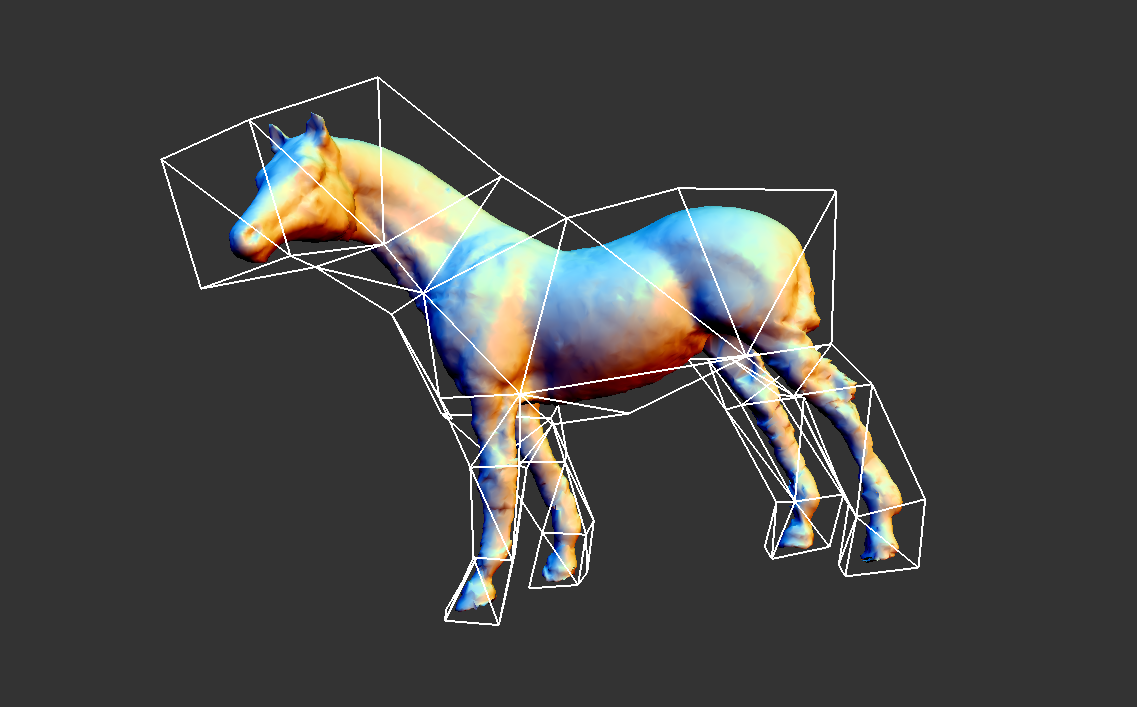
\includegraphics[width=0.5\textwidth]{horse}
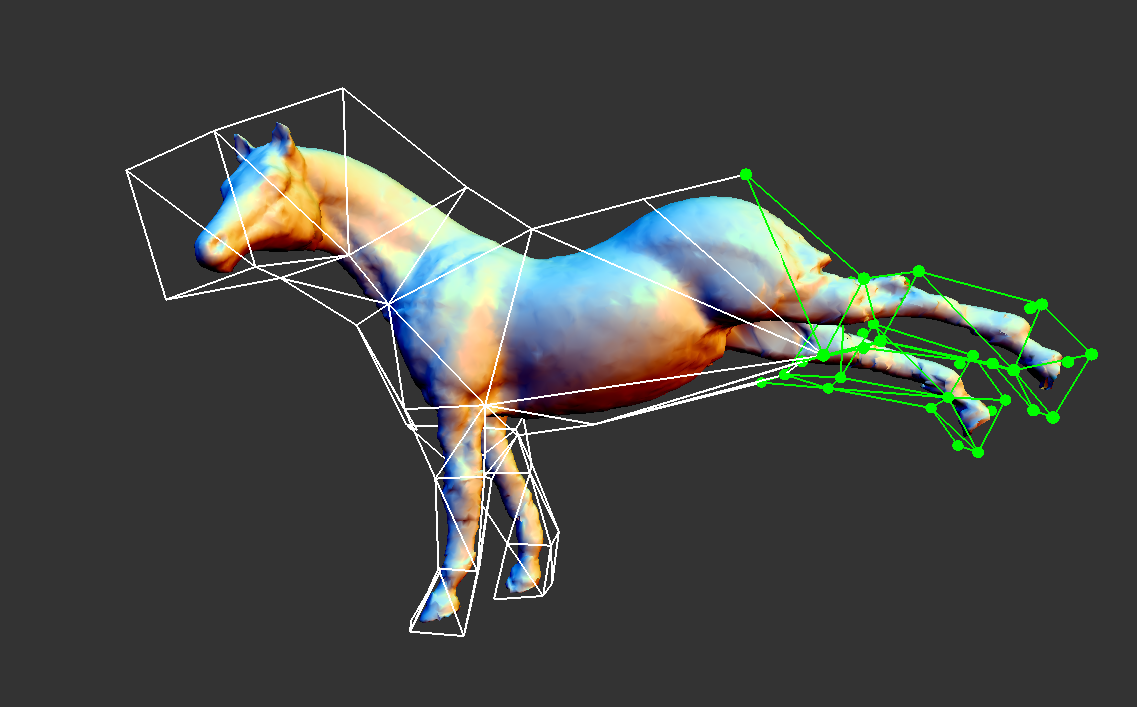
\includegraphics[width=0.5\textwidth]{horse_modified}

\end{frame}

\begin{frame}{Principes}

\begin{columns}

	\begin{column}{.7\textwidth}
	
\begin{itemize}
\item Maillage complexe
	\begin{itemize}
		\item[$\rightarrow$]Contrôle simple nécessaire
	\end{itemize}
\item Déplacement cage $\rightarrow$ cible
\end{itemize}

	\end{column}

	\begin{column}{.3\textwidth}
		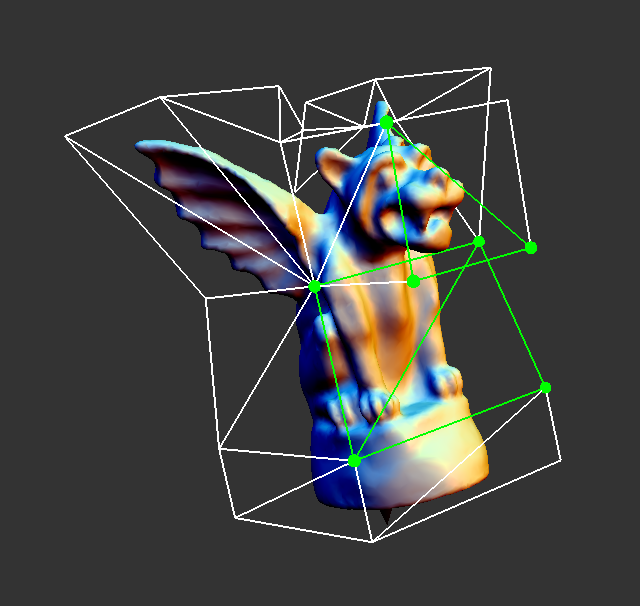
\includegraphics[width=\textwidth]{gargoyle}
	\end{column}
\end{columns}
\begin{block}{Maillage cible dans le \textit{repère} de la cage}
\begin{equation}
\label{eq:linear}
\mathbf{\eta} = \sum_{\mathbf{v_i} \in \mathbb{V}} \phi_i \left( \mathbf{\eta} \right) \mathbf{v_i} 
+ \sum_{t_i \in \mathbb{T}} \psi_i \left( \mathbf{\eta} \right) \mathbf{n} \left( t_i \right)
\end{equation}

\begin{equation}
\label{eq:def}
\mathbf{\eta'} = \sum_{\mathbf{v'_i} \in \mathbb{V}'} \phi_i \left( \mathbf{\eta} \right) \mathbf{v'_i} 
+ \sum_{t'_i \in \mathbb{T}'} \psi_i \left( \mathbf{\eta} \right) s \left(t'_i, t_i \right) \mathbf{n} \left( t'_i \right)
\end{equation}
\end{block}

\end{frame}


\begin{frame}{Déformation}
Quel système de coordonnées choisir ? Physiquement plausible
\begin{columns}
	\begin{column}{.8\textwidth}
%\begin{itemize}
%\item Quelles coordonées choisir ?
%\item Similitude $\rightarrow$ cage $\Leftrightarrow$ simitude $\rightarrow$ maillage
%\item Physiquement plausible
%\end{itemize}

\begin{block}{Coordonnées de Green}
\begin{equation}
\left\lbrace
\begin{array}{lcr}
\Delta \mathrm{Id} &=& 0 \\
\iiint_D \mathrm{div} \left( u \right)\,\mathrm{d}V &=& \iint_{\partial D} u \cdot \mathbf{n}\,\mathrm{d}\sigma
\end{array}
\right.
\end{equation}
\end{block}

\begin{itemize}
\item[$\Rightarrow$] Expression explicite des $\phi_i$, $\psi_i$
\item $\Delta \phi_i = \Delta \psi_i = 0$
\item Déformation du maillage $\mathcal{C}^\infty$ et \alert{quasi-conforme}
\item Variation locale des angles : \alert{borné}
\end{itemize}
	\end{column}
	\begin{column}{.2\textwidth}
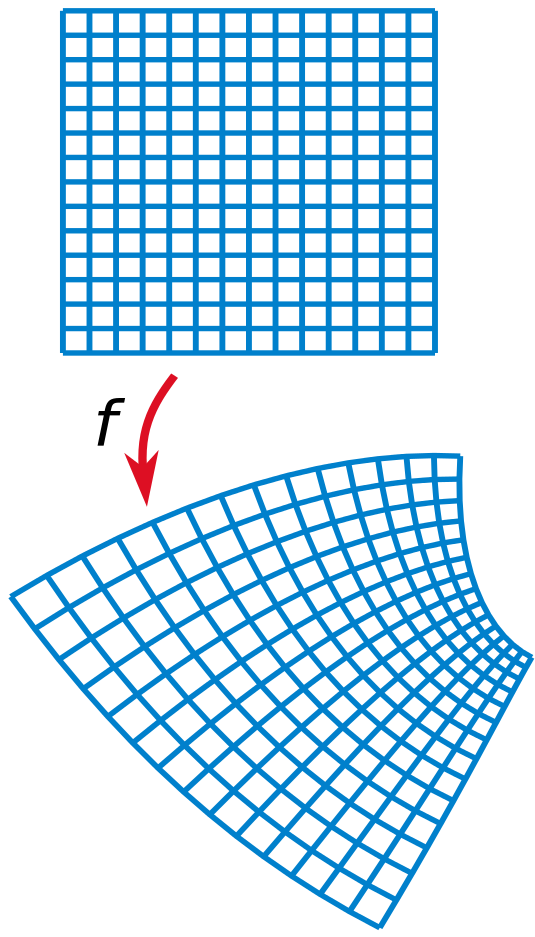
\includegraphics[width=\textwidth]{conformal}
	\end{column}
\end{columns}

\end{frame}

\begin{frame}{Programme}

\begin{block}{Fonctionnalités}
\begin{itemize}
\item Charge cage et maillage
\item Sélection des éléments de la cage
\item Translation, rotation, homothétie
\item Mise à jour de la cage en temps réel
\item Sauvegarde
\end{itemize}
\end{block}

\alert{Démonstration}

\end{frame}

\begin{frame}{Programme}
\begin{block}{Optimisation}
\begin{itemize}
\item Mise à jour en ligne du maillage cible
\begin{itemize}
\item Complexité $\leftarrow$ nombre d'éléments sélectionné
\end{itemize}
\item Parallélisation
\begin{itemize}
	\item \textit{Embarassingly parallel}
	\item \texttt{OpenMP}
	\item GPU ?
\end{itemize}
\end{itemize}
\end{block}
\end{frame}

\begin{frame}{Conclusion}
\begin{center}

\includegraphics[width=0.7\textwidth]{ratatouille}
\end{center}
Questions ?
\end{frame}
\end{document}

